\documentclass{article}

\usepackage{graphicx}
\usepackage{amsmath,amssymb,bm}
\usepackage{tikz}
\usepackage{pgfplots}
\pgfplotsset{compat=1.18}
\usetikzlibrary{calc,angles,quotes}
% Bold vectors for Latin and Greek:
\newcommand{\vect}[1]{\bm{#1}}    % \vect{x}, \vect{\alpha}, \vect{\nabla}
\newcommand{\uvect}[1]{\hat{\bm{#1}}} % unit vectors: \uvect{n}

\author{Thomas Dizon}
\title{CPU Graphics Engine}

\begin{document}

\maketitle

\begin{figure}[h]
	\centering
	\includegraphics[width=0.6\textwidth]{scene.png}
	\caption{}
\end{figure}

\newpage

\tableofcontents

\newpage

\section{Introduction}

\subsection{Motivation}
\begin{itemize}
\item As someone interested in developing 3D games and graphics, I was frustrated with how much I didn't understand when I used game engines like Unity and Godot. When I wanted to achieve a simple effect like adding grass, water or natural-looking terrain, I was overwhelmed with my own inability. Thus, I committed myself to building a 3D engine from scratch so I could allow these concepts that I didn't understand emerge naturally as byproducts as I worked towards the goal of rendering 3D objects. 
\item Now that I've more or less finished the project, it is A LOT easier now to imagine how to achieve some graphical effect like a grass or water shader. Since I understand how it works conceptually under the hood, the programming is a lot easier.
\item It's also a great precursor to understanding more in depth how the GPU works.
\end{itemize}

\subsection{What is a \textit{Graphics Engine}?}
\begin{itemize}
\item The 'rasterization' step in the graphics render pipline is a specific part which involves converting Primitives into Fragments
\item A primitive, in my case, is a Triangle and a Fragment is an (x,y) value on the screen with an additional z value to track its depth
\item In the real world, rasterization is done purely through specialized hardware on the GPU (which is why it is so fast)
\item To conceptually understand how it works, instead of building a GPU from scratch (hard), I'll use my good old CPU to do the rasterizing (still hard but easier)
\end{itemize}

\subsection{Why \textit{C}?}
\begin{itemize}
\item I first touched C during my Systems Programming course at University. It was extrememly difficult for me at the time but very benefiical for my programming skills. I felt that I haven't extracted all that I can from the language yet.
\item Also, I wanted to get as low level as possible for this project to ensure I had minimal dependencies. To truly understand the Graphics Pipeline, I wanted to build it truly (well, mostly) from scratch
\end{itemize}

\subsection{What does the project depend on?}
\begin{itemize}
\item Right now, it depends on the C standard library, std\_image.h (reference) for dealing with .png files and SDL2 (reference) for handling all the OS level stuff like inputs and writing to the screen. Though you could easily replace SDL with any other library which creates Windows for you like RayLib.
\end{itemize}

\section{The Graphics Pipeline}
\subsection{Diagram}
\subsection{Overview}
\begin{itemize}
\item{Primitive Assembly}
\item{Vertex Shader}
\item{Clipping \& Viewport}
\item{Rasterization}
\item{Fragment Shader}
\item{Output Merging \& Depth Test}
\end{itemize}

\section{3D Geometry in Memory}

\subsection{How do you represent a 3D object on a computer?}
\subsubsection{Vertices and Triangles}
\begin{itemize}
\item Using a Mesh
\end{itemize}
\subsubsection{3D Mesh}
\subsection{3D File types}

\section{Coordinate Spaces}
\subsection{What is a \textit{Coordinate Space}?}
\subsection{GameObjects \& Object Space}
\subsection{Scenes \& World Space}
\subsection{Cameras \& View Space}

\section{Transforming Vertices}
\subsection{Why do we need 4 dimensions?}
\subsection{Matrices as Transformations}
\subsection{Quaternions as Rotations}
\subsection{The Model Matrix}
\subsection{The View Matrix}
\subsection{The Projection Matrix}
\subsection{The Viewport Matrix}
\subsection{The Vertex Shader}
\subsection{Clipping \& The Sutherland Hodgman Algorithm}

\section{Drawing to the screen}
\subsection{What is \textit{Rasterization}?}
\subsection{Interpolation}
\subsection{Barycentric Coordinates}
\subsection{Rasterizing Triangles}
\subsection{What is a \textit{Fragment?}}
\subsection{The Fragment Shader}

\section{Shading}

\subsection{Materials}
\begin{itemize}
	\item A Material
	\item It contains ...
\end{itemize}

\subsection{Textures}
\subsection{Unlit Shader}
\subsection{Lit Shader}
\subsection{Phong Shader}
\subsection{Toon Shader}
\subsection{Shadows}
\subsection{Ambient Occlusion}

\section{Deprecated}
\subsection{Math Concepts}
\subsubsection{Vectors}
\begin{itemize}
\item In this document, we will use typical Vector operations and notation including but not limited to the following
\item A vector is $\textbf{v}$ is a collection of real numbers denoted by 
\item The \textit{dot product} is defined by
\item The \textit{cross product} is defined by
\item A unit vector is denoted by the hat
\end{itemize}

\subsubsection{Planes}
\begin{itemize}
	\item A plane is defined by \textbf{**TODO**}
\end{itemize}
\subsubsection{Matrices}

\begin{itemize}
	\item To understand Graphics Engines, you must become somewhat familiar with the operation of matrices. In particular: Matrix Multiplication, Inverse Matrices, Matrices as Linear Transformations and probably more. I provide a very scarce review below.
	\item Matrix multiplication is done like so:
	\item Matrix Inverse is calculated like so:
	\item For an affine, orthonormal matrix, the inverse can be calculated like this ( + reference)
\end{itemize}
\subsubsection{Quaternions}
\begin{itemize}
	\item To represents rotations in 3D space, I use Quaternions. While you can use a composition of 3x3 Euler Matrices, they are slower, hard to interpolate and are at risk of Gimbal Lock (+ Reference).
	\item A Quaternion is a kind of 4D complex number $q = q_0 + q$ where $q_0$ is a scalar and
$q$ is an R3 vector where each component has unit vectors $i, j, k$.
	\item The unit vectors $i,j,k$ adhere to the following multiplication rules. \textbf{**TODO**}
	\item Whenever you are interested in rotating an object in 3D space, you need to specify 2 things: An axis and an angle. These are encoded in the Unit Quaternion in the following way: \textbf{**TODO**}
	\item In the space of Unit Quaternions, if you operate a Unit Quaternion on a Vector, it results in a rotation of some degrees about some axis.
\end{itemize}
\subsubsection{Coordinate Spaces}
\begin{itemize}
	\item Cartesian
	\item Projective
	\item Barycentric
	\item Spherical, Cylindrical
\end{itemize}
\subsubsection{Transformations}
\begin{itemize}
	\item Model, View, Projection
\end{itemize}
\subsubsection{Deriving the Model Matrix}
\subsubsection{Deriving the View Matrix}
\subsubsection{Deriving the Projection Matrix}

The Projection Matrix is responsible for converting vertices from View space into Clip space. It aims to morph points that lie inside or on the View frustum into the Canonical View Volume in such a way that \textit{perspective} is introduced.  

\par\medskip
Perspective is described simply by the idea that things that are far away seem small and things that are close seem big.

\par\medskip
We break the problem  up into 2 parts:
\begin{enumerate}
	\item Calculating the transformation for $x$ and $y$
	\item Calculating the transformation for $z$
\end{enumerate}

For the first part, consider the setup in Figure \ref{fig:frustum}. In this 2D slice, the viewing volume is given by the near and far planes and the top and bottom planes. What we wish to do is to take some point $v$, and project it onto the near plane. 

To do this, we draw a line from the point to the origin. Consider the point at which this origin ray intersects the near plane. Let's call this point $x$. 


\begin{figure}[h!]

	\centering
	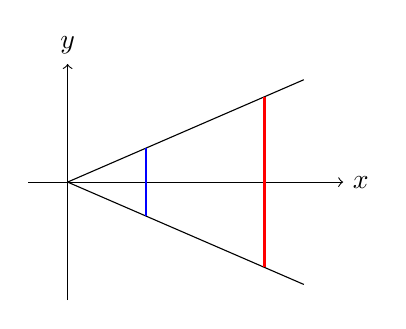
\begin{tikzpicture}[]

		%axis%
		\draw[->] (-0.5,0) -- (3.5,0) node[right] {$x$};
		\draw[->] (0,-1.5) -- (0,1.5) node[above] {$y$};

		% top plane %
		\draw (0,0) -- (3,1.3);

		% bottom plane %
		\draw (0,0) -- (3,-1.3);

		% near plane
		\draw[thick, blue] (1,0.43) -- (1, -0.43);

		% far plane %
		\draw[thick, red] (2.5, 1.08) -- (2.5, -1.08);

	\end{tikzpicture}
	\caption{2D slice depicting the top, bottom, near and far planes}
	\label{fig:frustum}
\end{figure}

\subsubsection{Deriving the Viewport Matrix}
\subsection{Algorithms}
\subsubsection{Rasterization}
\subsubsection{Improved Rasterization}
\begin{itemize}
	\item (First Approach) Takes a Primitive (Triangle made of Vertices) after is has been transformed by MVP and VP. It computes Bounding Box and using BaryCentric Coordinates with respect to the Triangle vertex positions decides which pixels to remove based on whether they are inside or outside of the triangle \textbf{**FIGURE**}
	\item (Optimized Approach) Iterative Edge Functions \textbf{**TODO**}
\end{itemize}

\subsubsection{Clipping}
\begin{itemize}
	\item After the Vertex Shader is applied, triangle vertices should be in \textit{Clip Space}, which is a \textit{homogeneous vector space} in $R^4$ where $v = (x,y,z,w)$ maps to $u = (x/w, y/w, z/w)$ in $R^3$
	\item The goal of this algorithm is to \textit{clip} the triangle against the \textit{View Frustum}, which in homoegenous space is a volume bounded by 6 4D planes.
	\item We start by deriving an expression for each planes, represented by a normal vector $n \in \mathbb{R}^4$ and some point on the vector $p \in \mathbb{R}^4$
	\item The projection matrix maps each of the 6 $\mathbb{R}^3$ planes that define the view frustum. \textbf{**TODO**} Show that the 6 view frustum planes map to the planes used in 4 space

\item \textbf{**TODO**} Write some pseudocode, include a diagram

\end{itemize}
\section{Conclusion \& Future Work}

\subsection{What I learnt}

\subsection{Limitations}

\subsection{A future implementation in C++}


\section{References}

\end{document}

